\chapter{Componentes de la propuesta}

En este capítulo se presentan los componentes, es decir, las funcionalidades propias de los algoritmos que se utilizaran como base (presentados en el capítulo anterior). 
Se describirán detalladamente además de usar pseudocódigo para representarlos.

\section{Componentes comunes}

\subsection{Operador de Reparación}

Cuando se realiza el cruce de dos soluciones pueden ocurrir dos casos:
\begin{itemize}
	\item El resultado del cruce pueda seguir considerándose una solución.
	\item El resultado del cruce no constituya el espacio de soluciones.
\end{itemize}

Más adelante en este capítulo se explicarán cómo son los cruces y se entenderá por qué es posible que el resultado de un cruce no sea una solución. 
En este caso, no es lógico desechar al ``hijo'', por lo que debemos ``arreglarlo'' para que se vuelva una solución. 
Ese es el objetivo del Operador de Reparación. 

En nuestro caso lo vamos a aplicar en ambos casos (que el ``hijo'' sea solución o no). 
Si el ``hijo'' no es solución es obvio el por qué necesitamos aplicarlo. 
Si el ``hijo'' es solución lo aplicaremos para asegurarnos que no hay huecos libres, es decir, que no hay elementos adicionales que podrían introducirse adicionalmente. 
Esto último se hace ya que queremos maximizar el valor de la solución, por lo que si queremos que sea mínimamente competente para cuando intentemos introducirlas en la población. 

Entonces seguimos el siguiente proceso, ilustrado en el pseudocódigo \ref{alg:OR}:
\begin{itemize}
	\item Si no es solución (su peso supera al peso máximo): Se deberán eliminar elementos del ``hijo'' hasta que constituya una solución. 
La forma de eliminar elementos será usando Greedy, es decir, se eliminarán los elementos con menor proporción $valor\_acumulado/peso$. 
Esta lógica viene dada por un intento de eliminar el máximo peso posible sin reducir mucho el valor final cuando se vuelva una solución. 
	
	\item Si es solución (su peso no supera al peso máximo): Se buscará, utilizando Greedy, un elemento para introducir. 
En este caso, nos interesa encontrar el elemento con mayor proporción $valor\_acumulado/peso$, ya que eso nos permitiría potencialmente aumentar significativamente el valor total (evaluación de la función \textit{fitness}) de la solución. 
Esto es, al tener en cuenta el peso puede llegar a resultar en que seamos capaces de introducir más elementos, pudiendo superar finalmente el valor que se tendría si se introdujese el elemento con el mayor valor acumulado pero no permitiese introducir más elementos. 
Este proceso se repetirá hasta que no sea capaz de introducir ningún otro elemento en la solución. 
%Además, este caso también se aplica cuando se acaba el caso contrario, para asegurarnos que no se puede aumentar más el valor sin volver a superar el peso máximo. 
\end{itemize}


\begin{algorithm}[H]
\caption{Operador de Reparación}\label{alg:OR}
\begin{algorithmic}[1]
\Procedure \texttt{Operador Reparación}($hijo$)
\State Calcular el peso total de $hijo \xrightarrow{}{}$ \texttt{pesoHijo}
\If{\texttt{pesoHijo} > \texttt{c}}
	\While{\texttt{pesoHijo} > \texttt{c}}
		\State Eliminar elemento usando Greedy
	\EndWhile
\Else
	\State \texttt{anadido = true} 
	\While{\texttt{anadido}}
		\State \texttt{anadido} = Añadir elemento usando Greedy
	\EndWhile
\EndIf
\EndProcedure
\end{algorithmic}
\end{algorithm}

Téngase en cuenta que al eliminar y añadir elementos del ``hijo'', se debe recalcular su peso total.


\section{Componentes de AG}

\subsection{Cruce Uniforme}

El cruce es un operador genético usado para variar los cromosomas de una generación a otra. 
Dos soluciones obtenidas de la población con anterior se cruzarán con el objetivo de producir una descendencia superior. 

Nos encontramos con distintos tipos de cruces básicos:
\begin{itemize}
	\item \textbf{Cruce en un punto}:  Dados dos padres, se le asignan los elementos de \texttt{padre$_1$} a \texttt{hijo$_1$} y de \texttt{padre$_2$} a \texttt{hijo$_2$} hasta cierto cromosoma elegido con anterioridad. 
A partir de dicho cromosoma, cambiaremos la asignación de forma que \texttt{hijo$_1$} hereda de \texttt{padre$_2$} e \texttt{hijo$_2$} hereda de \texttt{padre$_1$}. 
Un ejemplo de este tipo de cruce podría ser:

\begin{figure}[H]
%     \centering
%     \begin{subfigure}[b]{0.3\textwidth}
%         \centering
%         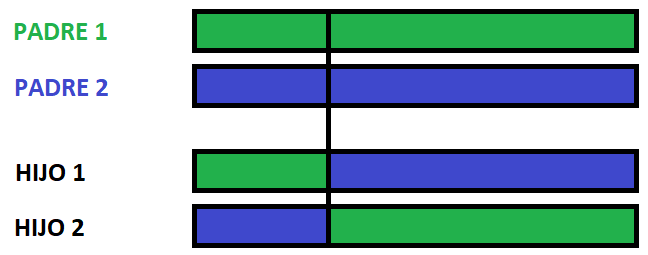
\includegraphics[scale=0.5]{imagenes/Crossover1point.png}
%%         \caption{$y=x$}
%         \label{fig:Crossover1point}
%     \end{subfigure}
%     \hfill
%     \begin{subfigure}[b]{0.3\textwidth}
%         \centering
%         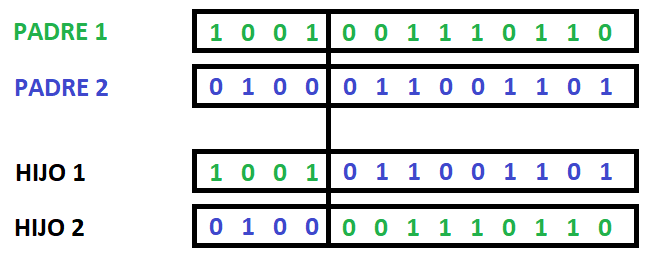
\includegraphics[scale=0.5]{imagenes/Crossover1pointNumber.png}
%%         \caption{$y=3\sin x$}
%         \label{fig:Crossover1pointNumber}
%     \end{subfigure}
		\centering
		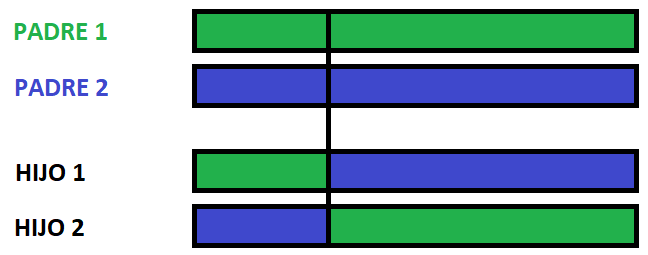
\includegraphics[scale=0.5]{imagenes/Crossover1point.png}
		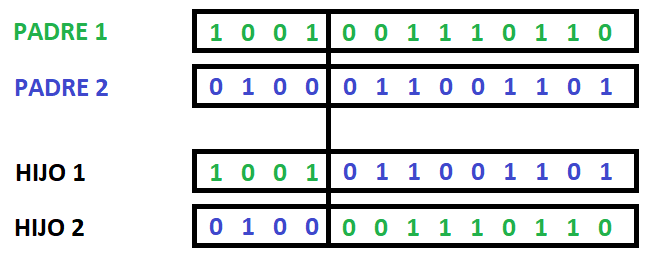
\includegraphics[scale=0.5]{imagenes/Crossover1pointNumber.png}
        \caption{Cruce en un punto}
        \label{fig:Crossover1}
\end{figure}

	\item \textbf{Cruce en dos puntos}: Sigue la misma lógica que el anterior, solo que elegimos dos puntos a partir de los cuales se cambian los elementos de qué padre se asignan a cada hijo. 
Un ejemplo de este tipo de cruce podría ser:
\begin{figure}[H]
		\centering
		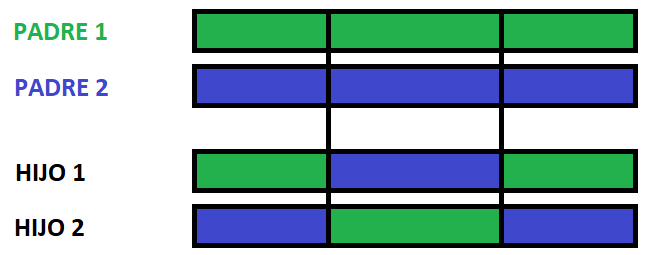
\includegraphics[scale=0.5]{imagenes/Crossover2point.png}
		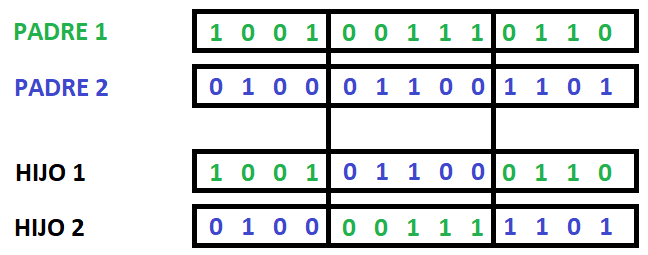
\includegraphics[scale=0.5]{imagenes/Crossover2pointNumber.png}
        \caption{Cruce en dos puntos}
        \label{fig:Crossover2}
\end{figure}
	\item \textbf{Cruce uniforme}: En este caso, en cada cromosoma se elige de forma aleatoria de qué padre lo hereda, cumpliéndose que si un hijo hereda cierto cromosoma de un padre, el otro hijo deberá heredar el mismo cromosoma del otro padre. 
Un ejemplo de este tipo de cruce sería: 
\begin{figure}[H]
		\centering
		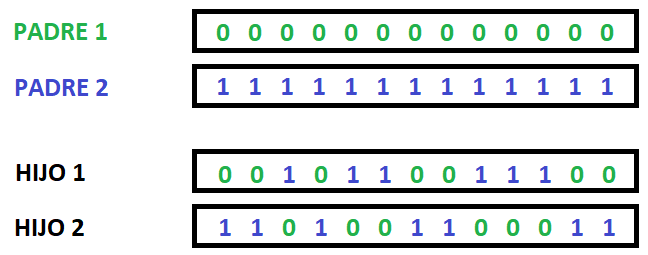
\includegraphics[scale=0.5]{imagenes/CrossoverUniformNumber.png}
        \caption{Cruce Uniforme}
        \label{fig:CrossoverUniform}
\end{figure}
\end{itemize}

El cruce de dos soluciones buenas no tiene por qué siempre dar lugar a una solución mejor o igual de buena. 
Sin embargo, si los padres son buenas soluciones, la probabilidad de tener un hijo bueno es elevada; en el caso de que el hijo no sea una buena solución, será eliminado durante el periodo de reemplazo. 

En nuestro problema es posible que el cruce de dos soluciones no de lugar a una solución. 
Esto se debe a la elección aleatoria de qué cromosomas elegir, no estamos teniendo en cuenta el peso que se está alcanzando al asignar cada elemento; por lo que es totalmente posible que  al asignar los elementos a cada hijo se sobrepase la capacidad máxima, dejando por ello de ser una solución válida. 

%Más adelante en este capítulo explicaremos otro tipo de cruce, que es el cruce HUX. 

En nuestro caso, realmente utilizamos una mezcla de cruce en un punto y cruce uniforme. 
Esto es, vamos a asignarle a cada hijo la mitad de cada uno de los padres, pero esta asignación será aleatoria: desordenamos el orden de los índices y lo partimos por la mitad. 
Esto viene representado en el pseudocódigo (\ref{alg:CU}) siguiente

\begin{algorithm}[H]
\caption{Cruce Uniforme}\label{alg:CU}
\begin{algorithmic}[1]
\Procedure \texttt{Cruce Uniforme}($padre_1, padre_2$)
\State Desordenar los índices que indican la posición de cada elemento
\For{i in 0..$n$}
	\If{i < $n/2$}
		\State \texttt{hijo$_1$[indice[i]]} = \texttt{padre$_1$[indice[i]]}
		\State \texttt{hijo$_2$[indice[i]]} = \texttt{padre$_2$[indice[i]]}
	\Else
		\State \texttt{hijo$_1$[indice[i]]} = \texttt{padre$_2$[indice[i]]}
		\State \texttt{hijo$_2$[indice[i]]} = \texttt{padre$_1$[indice[i]]}
	\EndIf
\EndFor
\EndProcedure
\end{algorithmic}
\end{algorithm}

\subsection{Mutación}

Los primeros intentos de mezclar computación y evolución no progresaron porque pusieron énfasis en los textos de biología del momento y confiaban más en la mutación que en el cruce para generar nuevas combinaciones de genes. 

La mutación consiste en modificar al azar una muy pequeña parte del cromosoma de los individuos, y permite alcanzar zonas del espacio de búsqueda que no estaban cubiertas por los individuos de la población actual. 
La mutación sola de por sí generalmente no permite avanzar en la búsqueda de una solución, pero nos garantiza que la población no va a evolucionar hacia una población uniforme que no sea capaz de seguir evolucionando. 

De forma similar a lo explicado en el Operador de Reparación, una vez que obtengamos la nueva solución debemos comprobar si podemos introducir más elementos, con el fin de maximizar el valor que puede llegar a tener. 
Esto también lo haremos siguiendo la misma lógica: ir introduciendo los genes con mayor proporción $valor\_acumulado/peso$.

\begin{algorithm}[H]
\caption{Mutación}\label{alg:Mutation}
\begin{algorithmic}[1]
\Procedure \texttt{Mutación}($poblacion$, $prob\_mut$)
\State Calcular el número de cromosomas que mutarán $\xrightarrow{}{}$ \texttt{nmut = $n$*prob\_mut}
\State Almacenar de forma aleatoria sin repetición \texttt{nmut} cromosomas de \texttt{poblacion} $\xrightarrow{}{}$\texttt{mutacion}
\For{i in 0..\texttt{nmut}}
	\State Elegir dos genes con distinto valor de forma aleatoria
	\If{Al intercambiar los genes sigue siendo válido}
		\State Intercambiar los genes
	\Else
		\State Volver al paso anterior
	\EndIf
	\State \texttt{anadido = true} 
	\While{\texttt{anadido}}
		\State \texttt{anadido} = Añadir elemento usando Greedy
	\EndWhile
	\State Calcular el valor de la función \textit{fitness}
\EndFor
\EndProcedure
\end{algorithmic}
\end{algorithm}

\subsection{Operador de Reemplazo Estacionario}

Una vez que hemos generado nuevas soluciones a partir del cruce de soluciones de la población existente, es necesario establecer un criterio sobre qué soluciones se mantienen o insertan en la población para la siguiente generación. 
En esta versión del Operador de Reemplazo el criterio que se sigue es el enfrentamiento de al población actual con las soluciones hijas, la población resultante estará compuesta de aquellos con mayor valor al calcular su función \textit{fitness}. 

En concreto, para lo que se aplica en el algoritmo base, AG, tenemos en cuenta que solo generamos 2 soluciones hijas antes de enfrentarlas con la población. 
Por ello, se ha optado por un método simplificado de enfrentamiento que consiste en encontrar cuáles son las 2 peores soluciones de la población actual (es decir, aquellas soluciones de la población actual con menor valor \textit{fitness}) y comprobar si las hijas son mejores o no. 
Se puede seguir su esquema en el pseudocódigo \ref{alg:ORE}. 
Usaremos los índices de forma que indique un orden de valores \textit{fitness}, por ejemplo, dados \texttt{padre$_1$} y  \texttt{padre$_2$}, se cumplirá que \textit{fitness}(\texttt{padre$_1$}) > \textit{fitness}(\texttt{padre$_2$}). 
Además, por conveniencia en la notación, se entenderá que \texttt{solucion$_i$} > \texttt{solucion$_j$} significa que el valor \textit{fitness} de \texttt{solucion$_i$} es mayor al de \texttt{solucion$_j$}.

Más adelante en la sección de ``Componentes de CHC'' de este capítulo se presenta la versión más generalizada de este tipo de enfrentamiento.

\begin{algorithm}[H]
\caption{Operador de Reemplazo Estacionario}\label{alg:ORE}
\begin{algorithmic}[1]
\Procedure \texttt{Op Reemplazo Estacionario}
\State Calcular los 2 peores padres de la población actual $\xrightarrow{}{}$ \texttt{padre$_1$}, \texttt{padre$_2$}.
\If{\texttt{hijo$_1$} > \texttt{padre$_1$} \&\& \texttt{hijo$_2$} > \texttt{padre$_2$}}
	\State Intercambiar ambas soluciones de la población por ambos hijos
\ElsIf{\texttt{hijo$_1$} > \texttt{padre$_2$}}
	\State Intercambiar la peor solución de la población por el mejor hijo
\Else
	\State No hacer nada, ya que los dos hijos son peores que las peores soluciones de la población
\EndIf
\EndProcedure
\end{algorithmic}
\end{algorithm}

\section{Componentes de CHC}

\subsection{Cruce HUX}

El cruce HUX (\textit{Half Uniform Crossover}) se caracteriza por, dados dos cromosomas, asignarle a los resultados del cruce en primer lugar los genes comunes a ambos padres y el resto de los genes serán repartidos a partes iguales entre ambos padres. 
Es decir, exactamente la mitad de los genes no coincidentes se intercambian en los hijos. 

A continuación se detallará en forma de pseudocódigo (\ref{alg:HUX}) el comportamiento de este tipo de cruce. 
Aunque primero se mostrará un ejemplo de este tipo de cruce:

\begin{figure}[H]
		\centering
		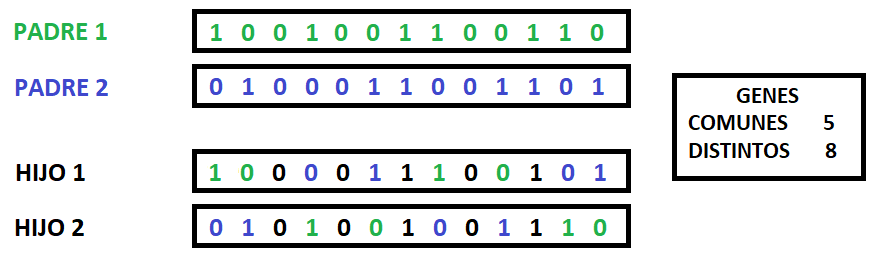
\includegraphics[scale=0.5]{imagenes/CrossoverHUX.png}
        \caption{Cruce HUX}
        \label{fig:HUX}
\end{figure}

\begin{algorithm}[H]
\caption{Cruce HUX}\label{alg:HUX}
\begin{algorithmic}[1]
\Procedure \texttt{Cruce HUX}($padre_1, padre_2$)
\State Asignar los genes comunes de los padres a ambos hijos
\State Desordenar los índices que indican la posición de cada gen restante $\xrightarrow{}{}$ Supongamos tamaño $m \leq n$
\For{i in 0..$m$}
	\If{i < $m/2$}
		\State \texttt{hijo$_1$[indice[i]]} = \texttt{padre$_1$[indice[i]]}
		\State \texttt{hijo$_2$[indice[i]]} = \texttt{padre$_2$[indice[i]]}
	\Else
		\State \texttt{hijo$_1$[indice[i]]} = \texttt{padre$_2$[indice[i]]}
		\State \texttt{hijo$_2$[indice[i]]} = \texttt{padre$_1$[indice[i]]}
	\EndIf
\EndFor
\EndProcedure
\end{algorithmic}
\end{algorithm}

\subsection{Enfrentamiento}

Es una generalización del Operador de Reemplazo Estacionario del AG. 
En este caso tenemos que enfrentar toda la población de hijos (con tamaño menor igual al tamaño de la población) contra toda la generación anterior. 
Por ello, no podemos seguir el método de obtener los $x$ peores elementos de la población para enfrentarlos con los hijos; así que optaremos por otro razonamiento. 


